\documentclass[conference,12pt]{IEEEtran}
\IEEEoverridecommandlockouts
\usepackage{cite}
\usepackage{amsmath,amssymb,amsfonts}
\usepackage{algorithmic}
\usepackage{graphicx}
\usepackage{textcomp}
\usepackage[table,xcdraw]{xcolor}
\usepackage{float}
\def\BibTeX{{\rm B\kern-.05em{\sc i\kern-.025em b}\kern-.08em
    T\kern-.1667em\lower.7ex\hbox{E}\kern-.125emX}}

\begin{document}

\title{The Exhaustion of IPv4 Address Space and the Transition to IPv6}

\author{
  \IEEEauthorblockN{Alexander Hoffmann}
  \IEEEauthorblockA{\textit{ECE Paris}\\
  Paris, France \\
  alexander.hoffmann@edu.ece.fr}
  \and
  \IEEEauthorblockN{Hugo Fougeres}
  \IEEEauthorblockA{\textit{ECE Paris}\\
  Paris, France \\
  hugo.fougeres@edu.ece.fr}
  \and
  \IEEEauthorblockN{Jeremy Roca}
  \IEEEauthorblockA{\textit{ECE Paris}\\
  Paris, France \\
  jeremy.roca@edu.ece.fr}
}

\maketitle

\section{Introduction}
At the beginning of networking, computer scientists were trying to determine the most efficient means of routing information so that it could be efficiently transmitted throughout the network. It was found that each connected computer maintains its own local address for the information it receives and that both the internetwork's most populous nodes (known as hubs) and the nodes connected to the most rural nodes do the same. Based on this information, and the IP version 4 address system was created. It uses 32 digital bits to represent addresses, generating a theoretical total limit of 4.3 billion addresses.

In May 2016 , International Internet Registration Authority (IARI), the authoritative organization for Internet numbering, declared the global Internet already fragmented. The IPv4 address space now supports only around 36,000 unique identifiers. At the rate of depletion, many, or even most, of the Internet's current home addresses could cease to exist within a decade. It is therefore not unrealistic to expect many existing IP-based applications and services to disappear from the internet at some time in the foreseeable future. It is likely that the first to go will be file sharing, but it is equally possible that other notable Internet-based services, such as online games, forums, instant messaging, and backup, will go in that order. Certain "workarounds" have been proposed to try to keep the web alive, such as re-using one-time addresses, mixing address pairs, and distributed denial of service. But the picture is grim.

Due to degradation in the availability of new IPv4 addresses, some of the community switched to IPv6. New trends in Internet innovation and increased usage of broadband make IPv6 an attractive choice. The most recent public audit, however, found that the Internet's IPv6 address space is still shrinking. In 2008, the Internet reached a global peak of IPv6 addresses.

This paper discusses the depletion of IPv4 addresses. The paper also reviews replacement strategies. Currently, IPv6 is the most widely cited replacement candidate for IPv4. This document analyses IPv6 as an example replacement and goes over technical and security components of IPv6.

\section{Internet Addressing}
The Internet Protocol (IP) is the dominant network protocol upon which many applications run.  This involves everything from Web browsing, to the stability of data communication, to the bandwidth efficient nature of broadband communications. There are many communication protocols, the most common of which are TCP and UDP. All of these protocols in turn use IP to translate between traffic types. Each Internet protocol is optimized for a particular purpose, such as routing packets and transferring data from point to point.

IPv4  was created in the early 1970s as an Internet Protocol that ran over the Department of Defense/US military, allowing secure messages between US Army "black sites". It offers a uniform solution to the problem of identifying hosts that should be allocated resources and to problems associated with timing and address inconsistencies. IPv4 addresses are 16-bit integers, and are generally 128 bits wide. For instance, an IP address can consist of eight characters (like e.g. 192.168.1.100). Each Internet service provider (ISP) has its own "Network Address Translation" (NAT) software.  It translates each IP address in the public Internet to its private.

In the late 1990s, however, someone suggested an expansion of the IP protocol. IPv6  was created in 2000, with over 4 million people at present using it, to replace IPv4. From a security point of view, IPv6 is considered to be far more secure than IPv4 and runs with a small amount of overhead and no external dependency for critical services such as e-mail. IPv6 makes possible new functionality, such as distributing source addresses and addressing requests within multicast groups (i.e. broadcasts), delivering many more addresses in more contexts, and enabling network topologies to be defined in terms of many subnets instead of a single large address block.

Internet routers route by breaking each IP address into a network number and a host number on that network. Each host on a network is assigned a number, and the router then puts those hosts together to form a single network that can be given a specific IP address. Routing protocols are clever: they figure out how to translate between network numbers and hosts, while keeping the IP address.

\section{IPv4 Address Shortage}
Internet growth is inextricably related to the expansion of IPv4 address space consumption. For nearly a decade, the Internet has grown rapidly across the world, and space limitations for the 32-bit IPv4 address have become severe. The increasing demand for IPv4 infrastructure will increase the cost of procuring and managing IPv4 address space, and give Internet Service Providers an incentive to procure and offer and offer more IPv4 capacity to their customers. Reports about the date at which the IPv4 address space will be exhausted vary. Fig. \ref{summary} represents a summary of some reports.
\begin{figure}
\begin{table}[H]
\centering
\begin{tabular}{|l|c|c|c|c|}
\hline
\rowcolor[HTML]{3166FF} 
\multicolumn{1}{|c|}{\cellcolor[HTML]{3166FF}Document}                                                                              & Issued                                              & Author                                                  & IANA pool                                                & RIR pool                                                 \\ \hline
\begin{tabular}[c]{@{}l@{}}The ISP Column\\ (How long have we \\ got?)\end{tabular}                                                 & \begin{tabular}[c]{@{}c@{}}Jul.\\ 2003\end{tabular} & \begin{tabular}[c]{@{}c@{}}Geoff \\ Huston\end{tabular} & 2021                                                & 2022                                                \\ \hline
\begin{tabular}[c]{@{}l@{}}IPv4 Address Report\\ (Potaroo)\end{tabular}                                                             & \begin{tabular}[c]{@{}c@{}}Dec.\\ 2005\end{tabular} & \begin{tabular}[c]{@{}c@{}}Geoff \\ Huston\end{tabular} & \begin{tabular}[c]{@{}c@{}}Jan.\\ 2013\end{tabular} & \begin{tabular}[c]{@{}c@{}}Jan.\\ 2016\end{tabular} \\ \hline
\begin{tabular}[c]{@{}l@{}}Internet Protocol\\ Journal \\ (A Pragmatic Report \\ on IPv4 Address \\ Space Consumption)\end{tabular} & \begin{tabular}[c]{@{}c@{}}Sep.\\ 2005\end{tabular} & \begin{tabular}[c]{@{}c@{}}Tony\\ Hain\end{tabular}     & 2009                                                & 2016                                                \\ \hline
\begin{tabular}[c]{@{}l@{}}The ISP Column\\ (Numerology)\end{tabular}                                                               & \begin{tabular}[c]{@{}c@{}}Nov.\\ 2005\end{tabular} & \begin{tabular}[c]{@{}c@{}}Geoff \\ Huston\end{tabular} & \begin{tabular}[c]{@{}c@{}}Jan.\\ 2012\end{tabular} & \begin{tabular}[c]{@{}c@{}}Mar.\\ 2013\end{tabular} \\ \hline
\end{tabular}
\end{table}
\caption{Summary of IPv4 exhaustion reports}
\label{summary}
\end{figure}

On 31 January 2011, the last two unreserved IANA /8 address blocks were allocated to APNIC according to RIR request procedures. This event can be observed on Fig. \ref{ipv4-exhaust}.
\begin{figure}[htbp]
\centerline{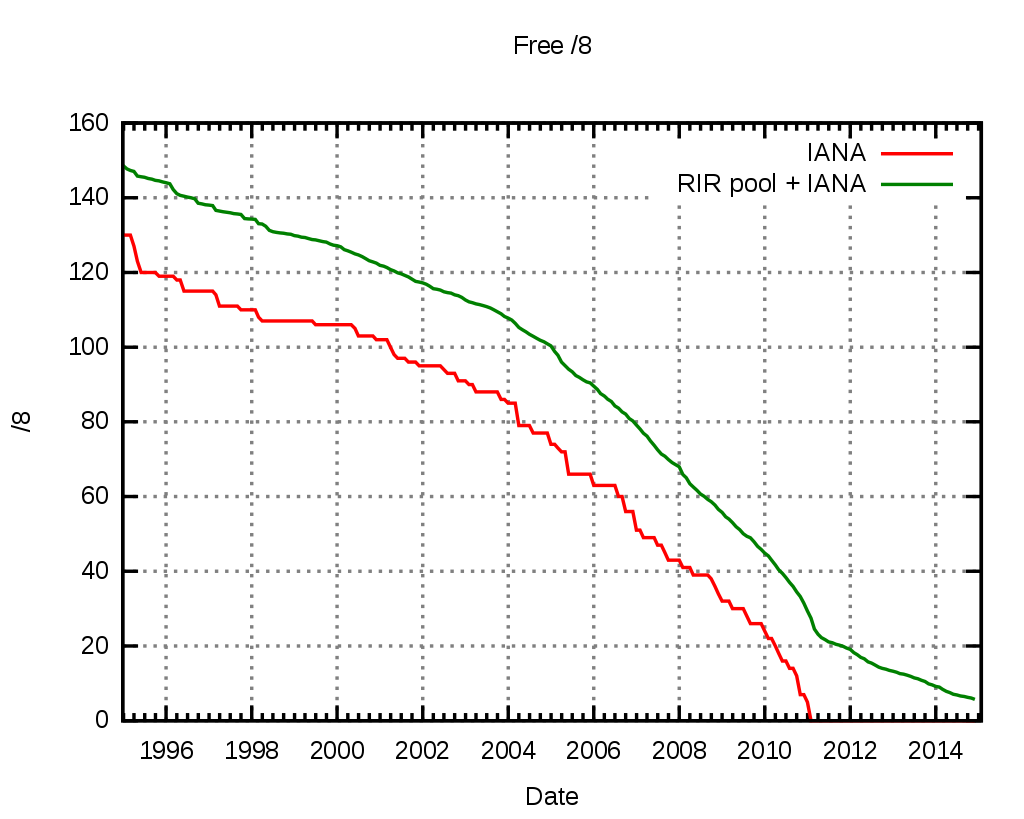
\includegraphics[scale=0.25]{resources/ipv4-exhaust.png}}
\caption{Exhaustion of IPv4 addresses since 1995}
\label{ipv4-exhaust}
\end{figure}

The IPv4 address space shortage had already been expected as early as 1990. Still, Fig. \ref{summary} shows how complex it was to predict the actual date of exhaustion. As of \today, there are a remaining 220.922/8 blocks of addresses available for public IPv4 Internet use. Fig. \ref{ipv4-current} shows the current status of the total IPv4 address space.
\begin{figure}[htbp]
\centerline{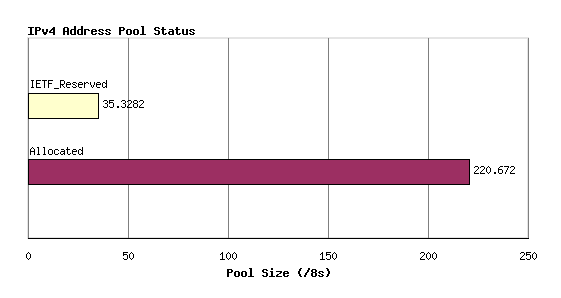
\includegraphics[scale=0.6]{resources/ipv4current.png}}
\caption{Address Pool Status}
\label{ipv4-current}
\end{figure}
The Regional Internet Registries (RIRs) control this allocated number pool. This is not a lot considering the speed at which the number of devices connected to the Internet is growing.

\section{Postponing the exhaustion of the IPv4 address space}

To delay the depletion of the number of networks, other technologies are employed such as Network Address Translation (NAT), Classless Inter-Domain Routing (CIDR), and Dynamic IPv4 Address Assignment (DHCP).

\subsection{NAT}
Network address translation (NAT) is a method of remapping one IP address space into another by modifying network address information in the IP header of packets while they are in transit across a traffic routing device. Networks in both public and private networks typically use the same "global" (universal) format, such as the single IPv4 address. Thus, since the address spaces have the same address format, NAT is not used to change the addresses in a network. NAT essentially changes the source of the packets by adding IP addresses which are slightly different, creating a unique network address for each incoming packet. This is considered to be the default method for routing internet content. It allows IP addresses from different geographic regions (US, Europe, Asia, Africa and the Middle East) to communicate on the same internet network. It is used most frequently to provide a connection between two remote networks. In this context, it is used to reduce the number of public IPv4 addresses used.

\subsection{CIDR}
Classless Inter-Domain Routing (CIDR) is a method for allocating IP addresses and IP routing. The key concept of CIDR is the concept of subnets for TCP and UDP packets. CIDR allows the router to partition its address space among multiple networks; however, because it first converts these networks into IP addresses, these networks are constantly being renegotiated as the default network/IP pair becomes redundant or outmoded. This method extends the IPv4 address space by assigning ULA addresses, whose size is three times larger than that of IPv4 addresses, and renumbering the 12 fully-qualified IPv4 CIDR blocks of IPv4 address space that are currently specified for use by the IPv4 multicast network. The three times larger ULA address space is intended to fulfill the needs of Internet routing throughout the space.\\

NAT and CIDR do not prevent the exhaustion of an IPv4 address, but in most cases the time taken to establish the new address is less than the expiration period. DHCP provides for simultaneous assignment of multiple addresses and is applicable when multiple hosts are configured to share the same IPv4 address in different subnets. All three use different techniques to extend the life of a network on the one hand, and to evade network address translation on the other.

The practical problem of limiting IPv4 addresses in order to minimize the number of addresses used cannot be solved using the techniques discussed in this section. It is uncertain when the end-of-life cutoff will be reached. Thus, despite of the recent industry efforts to achieve further growth in the capacity of IPv4 addressing, there is little evidence that IPv4 addresses can be produced, delivered, and utilized effectively enough to meet the future demand for IPv4 addressing.

\section{An alternative to IPv4: IPv6}
What is IPv6? IPv6 was first published in 1991 and it was intended to solve several serious problems in network communications, including enabling multipoint connections over a relatively small number of wire stations. At the most fundamental level, IPv6 takes the proven IPv4 protocol and extends the address space from 32-bits to 128-bits to accommodate traffic with ever-increasing sizes. This allows packets to be transferred at any speed. As of 2018, more than 65\% of Internet traffic is IPv6 and it is estimated that one in three websites utilize IPv6 to achieve a better experience for their users. IPv6 is designed to work with many different gateways, including DNS, router, and firewalls. It can provide faster, smoother broadband connections. This might be for online gaming, for downloading files, or just on social networking sites. Here are some of the features of IPv6:
\begin{itemize}
\item Enhanced applications functionality – Enables peer-to-peer, infrastructure-less applications and networking (vs. client-server model).
\item End-to-end transparency – Reduces motivations for address translation technologies.
\item Hierarchical addressing – Summarizes and manages routing table growth.
\item Auto-configuration – The unicast IPv6 addressing architecture uses one half of the address (64 bits) to embed IEEE extended unique identifiers (EUI-64) in each interface address. The use of globally unique EUI-64s on each interface allows systems to derive globally unique IPv6 addresses automatically from simple announcements from neighboring systems.
\item Scalability of multicast routing – IPv6 provides a much larger pool of multicast addresses with multiple scoping options.
\item Larger address space - IPv6 increases the IP address size from 32 bits to 128 bits.
\end{itemize}

\section{Security implications of IPv6}
The use of IPv6 has a variety of security implications. IPv6 is a secure protocol because it provides a link layer encryption and a self-signed certificate system that introduces improved security. It protects content and services from IP spoofing and neighbor leaks. In this section, we will list some IPv6 security components.

\subsection{IPsec}
Internet Protocol Security (IPsec) is implemented at the core of IPv6. It supports multiple layers of security, including authentication, encryption and MAC or MAC security. IPsec is a security protocol designed to be compatible with many protocols such as TCP, UDP, IP, and SSH, which can be used to secure any connection. IPsec allows secure remote access to applications and devices on the network. This protocol provides interoperable, high quality and cryptographically based security services for traffic at the IP layer. It is particularly suitable for applications that need confidentiality and integrity; it is a common element in client/server applications, networks and firewalls.

\subsection{Neighbor Discovery Protocol}
The Neighbor Discovery Protocol (NDP) is a peer-to-peer protocol used to determine the IP addresses of nodes on a local or remote network. It was first developed by Microsoft in 1989 in an effort to optimize its networking with an emphasis on fast network I/O and robustness. Using the Neighbor Discovery Protocol, the local network establishes a "listening post" for the Internet, called a Default Gateway, which forwards connections to their final destination.

NDP reduces, minimizes, or even eliminates the risk of most eavesdropping and network attacks by establishing secure links between networks. The NDP packet security protocol defines a message-based security protocol for secure communication, called IPsec. It provides protection of data, such as in the IP packet format, and is based on an extension of IP packet security.

\subsection{Cryptographically Generated Address}
In IPv6, a public signature key may be bound to an address. A Cryptographically Generated Address (CGA) is generated. It offers additional security protection for the discovery process for the IPv6 neighborhood router, and allows the user to have a "proof of ownership" for a particular IPv6 address. This concept allows the public key address to be used to authenticate requests for network address space, while avoiding restrictions related to the use of public-key cryptography for forwarding network address space.\\

Every new protocol will of course bring new security issues. For IPv6, this involves the lack of implementation maturity and is therefore highly likely to still contain many new vulnerabilities. IPv6 might thus be considered to be still in its infancy and there are certain potential risks that are due to take some time to be addressed. Hence the use of IPv6 is under continuous review. Thus it may take years before many of these security concerns are fully addressed.

\section{Transition from IPv4 to IPv6}
The transition from IPv4 to IPv6 is not a one-day step and involves a lot of changes in network structures with the use of IP addresses.  Most programs and devices using existing network technologies will need to be upgraded to operate over IPv6. This is especially true for big multi-purpose networks, where the external point-to-point links between hosts have to be converted to host-to-host links in order to make IPv4 work properly. So the next challenge to navigate is the set of policies and procedures that will have to be designed and built into networks to allow for this transition. One significant problem is that the two IP address formats aren't compatible and total conversion to IPv6 is a way off. The transition from IPv4 to IPv6 is a process aimed at the gradual replacement of IPv4 by IPv6 on the Internet.

In this section, we present some of the most widely used IPv6 transition mechanisms. An IPv6 transition mechanism is a technology which facilitates the transition of the Internet from the IPv4 infrastructure in use since 1983 to the IPv6 successor addressing and routing system.

\subsection{Stateless IP/ICMP Translation}
Stateless IP / ICMP Translation (SIIT) is a conversion between the IPv6 and IPv4 packet header formats. The SIIT method describes IPv6 address class called IPv4-translated addresses. This class of address matches all IPv4 packets addressed to an IPv4-only interface. In contrast to IPv6 address families, SIIT does not include IPv6 routes, since all IPv4 addresses fall outside the SIIT scope of distribution. Also, SIIT does not include classless addresses since the classless address format has not been developed to address router filtering of classless packets. SIIT has been widely adopted since it operates seamlessly and is free. SIIT has the following advantages over the RIPE naming convention: SIIT provides an option to use IPv4-translated addresses to define a sub-netting and mappings in IPv4; SIIT provides an option to explicitly remove IPv4-translated addresses from the addressing tree when the scope of the resulting network is not IPv6-only. Finally, SIIT allows IPv6 packet headers to be routed more easily in the Internet than IPv4 packet headers.

\subsection{Dual-Stack}
A dual-stack device is a device with network interfaces that can originate and understand both IPv4 and IPv6 packets. With the dual stack solution, every networking device, server, switch, router and firewall in an ISP's network will be configured with both IPv4 and IPv6 connectivity capabilities. The transition is driven by DNS. If a dual-stacked device queries the name of a destination and DNS gives it an IPv4 address, it sends IPv4 packets. If DNS responds with an IPv6 address, it sends IPv6 packets. To dual stack all of a network's devices, the interfaces need both an IPv6 and an IPv4 address. This raises the issue that the Internet has run out of IPv4 addresses, which is the main reason IPv6 is needed in the first place. It will be possible to keep surfing the Internet without wondering if the connection will stop working because of the IP address conversion.


\subsection{Tunnel broker}
The tunnel broker provides IPv4 Internet connectivity to endpoints by encapsulating IPv6 transit traffic in IPv4 Internet transport links, typically using the 6in4 tunnel broker transport protocol. 6in4 is an IPv4 transport network protocol (TCP) that enables traffic from the Internet to be routed via 6in4 transit tunnels that use 6in4 tunnel rings to ensure communication integrity. The use of 6in4 tunnels has limited operational requirements, but a large percentage of companies are using 6in4 as part of their tunnel mapping solution. Tunnel brokers often use a dual-stack design to enable IPv6 connectivity in both IPv4 and IPv6 stacks. In doing so, tunnel brokers are able to provide networks by maintaining encapsulated, restricted-to-nodes tunnels over IPv4 Internet transit links. IPv6 tunnel brokers allow each node in the tunnel to advertise the tunnel's location to other nodes in the tunnel, and then to deliver the tunnel's traffic.

\subsection{6rd}
6rd is a method to accelerate delivery of the IPv6 service through IPv4 Internet service provider (ISP) infrastructures. It uses stateless address mapping between IPv4 and IPv6 addresses and transmits IPv6 packets through automatic tunnels along the same optimized routes as IPv4 packets between customer nodes. This feature allows a customer to switch from IPv4 to IPv6 at their location without having to modify their networks and routers, and does not involve reconfiguration of customer's sites and services. This makes the router to router tunneling resistant and highly scalable.\\

There are various kinds of technologies that can be implemented such as dual stack, tunneling methods, and techniques for translation as depicted in Fig. \ref{ipv6-transition}. To ensure interoperability between IPv4 and IPv6, more than seventeen transformation technologies have been used and tested for communications between different networks.
\begin{figure}[htbp]
\centerline{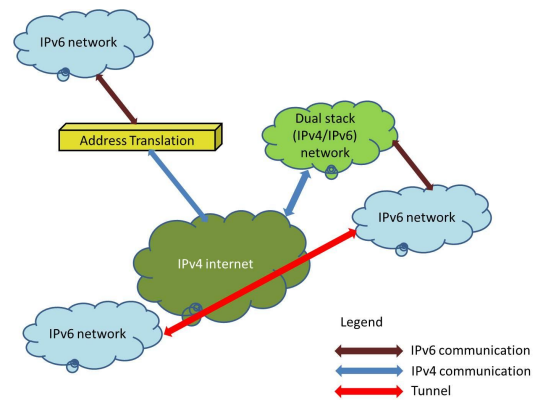
\includegraphics[scale=0.6]{resources/ipv6-transition.png}}
\caption{Different transition technologies}
\label{ipv6-transition}
\end{figure}
The National Internet System Consortium (NISCO) has conducted numerous research studies and workshops on protocol transition issues in both IPv4 and IPv6 and has identified a number of key parameters which should be considered when attempting to determine the feasibility of transition. These include network stability, reliability, security, test strategies, and deployment resources.

\section{Conclusion}
Although large, the number of addresses in the IPv4 address space is finite. IPv4 address space exhaustion  has been known since November 1999, when experts at the Internet Engineering Task Force (IETF) first warned of the problem. As a result, it has become urgent to find an alternative for IPv4. Currently, IPv6 is the most widely cited replacement candidate for IPv4. Using IPv6 has the advantage of lower latency, larger capacity, lower costs, and shorter time to service as compared to IPv4. On top of all, IPv6 is far more secure than IPv4 addresses, as it contains no extra ASCII characters. Furthermore, it provides a link layer encryption and a self-signed certificate system that introduces improved security.

However, implementing IPv6 efficiently is likely to present new challenges for Internet hosts and traffic sources. IPv6 is more difficult to configure, and is more complicated to use, than IPv4, although IPv6 implementations exist for many existing Internet standards. For this reason, IPv6 is under development, with an important goal of deployment during the next decade.

%%%% Bibliography %%%%

\begin{thebibliography}{9}
\bibitem{ieee-ipv4-exhaustion}
\textit{IPv4 Address Exhaustion, Mitigation Strategies and Implications for the U.S.}. 
Institute of Electrical and Electronics Engineers-United States of America. 2009.

\bibitem{icann-available-pool-ipv4}
\textit{Available Pool of Unallocated IPv4 Internet Addresses Now Completely Emptied}.
ICANN. 2011.

\bibitem{jpnic-ipv4-exhaustion}
\textit{Analysis and Recommendations on the Exhaustion of IPv4 Address Space}.
Japan Network Information Center. 2006.

\bibitem{ipv6}
S. Deering, R. Hinden.
\textit{Internet Protocol, Version 6 (IPv6) Specification}.
Internet Engineering Task Force. 2017.

\bibitem{ipv6-ripe}
\textit{IPv6 Address Allocation and Assignment Policy}.
RIPE NCC. 2011.

\bibitem{ipv6-security}
\textit{IPv6 Security}.
Government of the HKSAR. 2011.

\bibitem{ipv6-ndp}
\textit{Neighbor Discovery for IP version 6 (IPv6)}.
RFC 4861. 2007.

\bibitem{ipv6-ndp}
C. Partridge, F. Kastenholz
\textit{Technical Criteria for Choosing IP The Next Generation (IPng)}.
RFC 1726. 1994.

\bibitem{ipv6-ndp}
E. Nordmark, R. Gilligan
\textit{Basic Transition Mechanisms for IPv6 Hosts and Routers}.
RFC 4213. 2005.
\end{thebibliography}

\end{document}
